\PassOptionsToPackage{unicode=true}{hyperref} % options for packages loaded elsewhere
\PassOptionsToPackage{hyphens}{url}
\PassOptionsToPackage{dvipsnames,svgnames*,x11names*}{xcolor}
%
\documentclass[]{article}
\usepackage{lmodern}
\usepackage{amssymb,amsmath}
\usepackage{ifxetex,ifluatex}
\usepackage{fixltx2e} % provides \textsubscript
\ifnum 0\ifxetex 1\fi\ifluatex 1\fi=0 % if pdftex
  \usepackage[T1]{fontenc}
  \usepackage[utf8]{inputenc}
  \usepackage{textcomp} % provides euro and other symbols
\else % if luatex or xelatex
  \usepackage{unicode-math}
  \defaultfontfeatures{Ligatures=TeX,Scale=MatchLowercase}
\fi
% use upquote if available, for straight quotes in verbatim environments
\IfFileExists{upquote.sty}{\usepackage{upquote}}{}
% use microtype if available
\IfFileExists{microtype.sty}{%
\usepackage[]{microtype}
\UseMicrotypeSet[protrusion]{basicmath} % disable protrusion for tt fonts
}{}
\IfFileExists{parskip.sty}{%
\usepackage{parskip}
}{% else
\setlength{\parindent}{0pt}
\setlength{\parskip}{6pt plus 2pt minus 1pt}
}
\usepackage{xcolor}
\usepackage{hyperref}
\hypersetup{
            pdftitle={Module 9: Recommended Exercises},
            pdfauthor={Emma Skarstein, Daesoo Lee, Stefanie Muff; Department of Mathematical Sciences, NTNU},
            colorlinks=true,
            linkcolor=Maroon,
            filecolor=Maroon,
            citecolor=Blue,
            urlcolor=blue,
            breaklinks=true}
\urlstyle{same}  % don't use monospace font for urls
\usepackage[margin=1in]{geometry}
\usepackage{color}
\usepackage{fancyvrb}
\newcommand{\VerbBar}{|}
\newcommand{\VERB}{\Verb[commandchars=\\\{\}]}
\DefineVerbatimEnvironment{Highlighting}{Verbatim}{commandchars=\\\{\}}
% Add ',fontsize=\small' for more characters per line
\usepackage{framed}
\definecolor{shadecolor}{RGB}{248,248,248}
\newenvironment{Shaded}{\begin{snugshade}}{\end{snugshade}}
\newcommand{\AlertTok}[1]{\textcolor[rgb]{0.94,0.16,0.16}{#1}}
\newcommand{\AnnotationTok}[1]{\textcolor[rgb]{0.56,0.35,0.01}{\textbf{\textit{#1}}}}
\newcommand{\AttributeTok}[1]{\textcolor[rgb]{0.77,0.63,0.00}{#1}}
\newcommand{\BaseNTok}[1]{\textcolor[rgb]{0.00,0.00,0.81}{#1}}
\newcommand{\BuiltInTok}[1]{#1}
\newcommand{\CharTok}[1]{\textcolor[rgb]{0.31,0.60,0.02}{#1}}
\newcommand{\CommentTok}[1]{\textcolor[rgb]{0.56,0.35,0.01}{\textit{#1}}}
\newcommand{\CommentVarTok}[1]{\textcolor[rgb]{0.56,0.35,0.01}{\textbf{\textit{#1}}}}
\newcommand{\ConstantTok}[1]{\textcolor[rgb]{0.00,0.00,0.00}{#1}}
\newcommand{\ControlFlowTok}[1]{\textcolor[rgb]{0.13,0.29,0.53}{\textbf{#1}}}
\newcommand{\DataTypeTok}[1]{\textcolor[rgb]{0.13,0.29,0.53}{#1}}
\newcommand{\DecValTok}[1]{\textcolor[rgb]{0.00,0.00,0.81}{#1}}
\newcommand{\DocumentationTok}[1]{\textcolor[rgb]{0.56,0.35,0.01}{\textbf{\textit{#1}}}}
\newcommand{\ErrorTok}[1]{\textcolor[rgb]{0.64,0.00,0.00}{\textbf{#1}}}
\newcommand{\ExtensionTok}[1]{#1}
\newcommand{\FloatTok}[1]{\textcolor[rgb]{0.00,0.00,0.81}{#1}}
\newcommand{\FunctionTok}[1]{\textcolor[rgb]{0.00,0.00,0.00}{#1}}
\newcommand{\ImportTok}[1]{#1}
\newcommand{\InformationTok}[1]{\textcolor[rgb]{0.56,0.35,0.01}{\textbf{\textit{#1}}}}
\newcommand{\KeywordTok}[1]{\textcolor[rgb]{0.13,0.29,0.53}{\textbf{#1}}}
\newcommand{\NormalTok}[1]{#1}
\newcommand{\OperatorTok}[1]{\textcolor[rgb]{0.81,0.36,0.00}{\textbf{#1}}}
\newcommand{\OtherTok}[1]{\textcolor[rgb]{0.56,0.35,0.01}{#1}}
\newcommand{\PreprocessorTok}[1]{\textcolor[rgb]{0.56,0.35,0.01}{\textit{#1}}}
\newcommand{\RegionMarkerTok}[1]{#1}
\newcommand{\SpecialCharTok}[1]{\textcolor[rgb]{0.00,0.00,0.00}{#1}}
\newcommand{\SpecialStringTok}[1]{\textcolor[rgb]{0.31,0.60,0.02}{#1}}
\newcommand{\StringTok}[1]{\textcolor[rgb]{0.31,0.60,0.02}{#1}}
\newcommand{\VariableTok}[1]{\textcolor[rgb]{0.00,0.00,0.00}{#1}}
\newcommand{\VerbatimStringTok}[1]{\textcolor[rgb]{0.31,0.60,0.02}{#1}}
\newcommand{\WarningTok}[1]{\textcolor[rgb]{0.56,0.35,0.01}{\textbf{\textit{#1}}}}
\usepackage{graphicx,grffile}
\makeatletter
\def\maxwidth{\ifdim\Gin@nat@width>\linewidth\linewidth\else\Gin@nat@width\fi}
\def\maxheight{\ifdim\Gin@nat@height>\textheight\textheight\else\Gin@nat@height\fi}
\makeatother
% Scale images if necessary, so that they will not overflow the page
% margins by default, and it is still possible to overwrite the defaults
% using explicit options in \includegraphics[width, height, ...]{}
\setkeys{Gin}{width=\maxwidth,height=\maxheight,keepaspectratio}
\setlength{\emergencystretch}{3em}  % prevent overfull lines
\providecommand{\tightlist}{%
  \setlength{\itemsep}{0pt}\setlength{\parskip}{0pt}}
\setcounter{secnumdepth}{0}
% Redefines (sub)paragraphs to behave more like sections
\ifx\paragraph\undefined\else
\let\oldparagraph\paragraph
\renewcommand{\paragraph}[1]{\oldparagraph{#1}\mbox{}}
\fi
\ifx\subparagraph\undefined\else
\let\oldsubparagraph\subparagraph
\renewcommand{\subparagraph}[1]{\oldsubparagraph{#1}\mbox{}}
\fi

% set default figure placement to htbp
\makeatletter
\def\fps@figure{htbp}
\makeatother

\usepackage{etoolbox}
\makeatletter
\providecommand{\subtitle}[1]{% add subtitle to \maketitle
  \apptocmd{\@title}{\par {\large #1 \par}}{}{}
}
\makeatother

\title{Module 9: Recommended Exercises}
\providecommand{\subtitle}[1]{}
\subtitle{TMA4268 Statistical Learning V2022}
\author{Emma Skarstein, Daesoo Lee, Stefanie Muff \and Department of Mathematical Sciences, NTNU}
\date{March 14, 2022}

\begin{document}
\maketitle

\begin{center}\rule{0.5\linewidth}{0.5pt}\end{center}

\hypertarget{problem-1}{%
\subsection{Problem 1}\label{problem-1}}

Work through the lab in Section 9.6.1 of the course book.

\hypertarget{problem-2-book-ex.2}{%
\subsection{Problem 2 (Book Ex.2)}\label{problem-2-book-ex.2}}

We have seen that in \(p = 2\) dimensions, a linear decision boundary
takes the form \(\beta_0 +\beta_1 X_1 + \beta_2 X_2 = 0\). We now
investigate a non-linear decision boundary.

\begin{enumerate}
\def\labelenumi{\alph{enumi})}
\item
  Sketch the curve \[(1 + X_1)^2 + (2 - X_2)^2 = 4.\]
\item
  On your sketch, indicate the set of points for which
  \[(1+X_1)^2 +(2-X_2)^2 >4,\] as well as the set of points for which
  \[(1+X_1)^2 +(2-X_2)^2 \leq 4.\]
\item
  Suppose that a classifier assigns an observation to the blue class if
  \[(1+X_1)^2 +(2-X_2)^2 >4,\] and to the red class otherwise. To what
  class is the observation \((0, 0)\) classified?
  \((-1,1)?\quad (2,2)? \quad (3,8)?\)
\item
  Argue that while the decision boundary in (c) is not linear in terms
  of \(X_1\) and \(X_2\), it is linear in terms of \(X_1, X_1^2, X_2,\)
  and \(X_2^2.\)
\end{enumerate}

\hypertarget{problem-3}{%
\subsection{Problem 3}\label{problem-3}}

This problem involves plotting of decision boundaries for different
kernels and it's taken from
\href{https://www.youtube.com/watch?v=4KoL9vUI7xs\&list=PL5-da3qGB5IDl6MkmovVdZwyYOhpCxo5o\&index=5}{Lab
video}.

\begin{Shaded}
\begin{Highlighting}[]
\CommentTok{# code taken from video by Trevor Hastie}
\KeywordTok{set.seed}\NormalTok{(}\DecValTok{10111}\NormalTok{)}
\NormalTok{x <-}\StringTok{ }\KeywordTok{matrix}\NormalTok{(}\KeywordTok{rnorm}\NormalTok{(}\DecValTok{40}\NormalTok{), }\DecValTok{20}\NormalTok{, }\DecValTok{2}\NormalTok{)}
\NormalTok{y <-}\StringTok{ }\KeywordTok{rep}\NormalTok{(}\KeywordTok{c}\NormalTok{(}\OperatorTok{-}\DecValTok{1}\NormalTok{, }\DecValTok{1}\NormalTok{), }\KeywordTok{c}\NormalTok{(}\DecValTok{10}\NormalTok{, }\DecValTok{10}\NormalTok{))}
\NormalTok{x[y }\OperatorTok{==}\StringTok{ }\DecValTok{1}\NormalTok{, ] <-}\StringTok{ }\NormalTok{x[y }\OperatorTok{==}\StringTok{ }\DecValTok{1}\NormalTok{, ] }\OperatorTok{+}\StringTok{ }\DecValTok{1}
\KeywordTok{plot}\NormalTok{(x, }\DataTypeTok{col =}\NormalTok{ y }\OperatorTok{+}\StringTok{ }\DecValTok{3}\NormalTok{, }\DataTypeTok{pch =} \DecValTok{19}\NormalTok{, }\DataTypeTok{xlab =} \KeywordTok{expression}\NormalTok{(X[}\DecValTok{1}\NormalTok{]), }\DataTypeTok{ylab =} \KeywordTok{expression}\NormalTok{(X[}\DecValTok{2}\NormalTok{]))}
\end{Highlighting}
\end{Shaded}

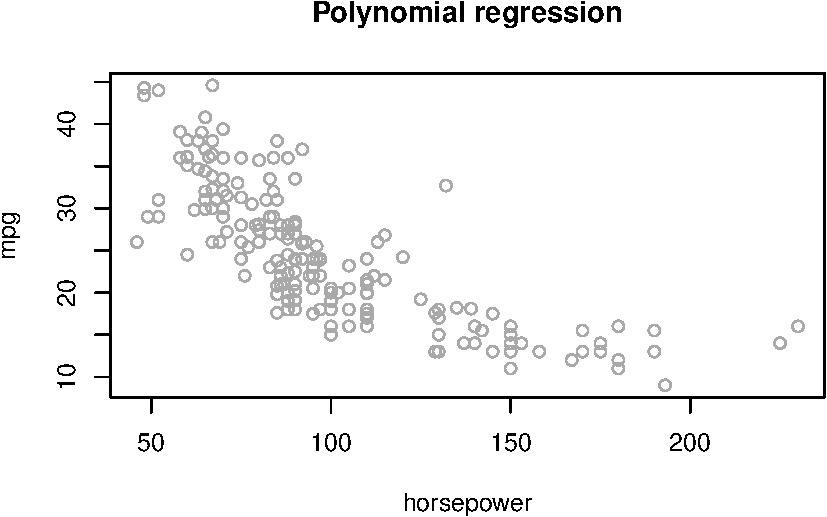
\includegraphics[width=0.5\linewidth]{RecEx9_files/figure-latex/unnamed-chunk-1-1}

\begin{Shaded}
\begin{Highlighting}[]
\NormalTok{dat =}\StringTok{ }\KeywordTok{data.frame}\NormalTok{(x, }\DataTypeTok{y =} \KeywordTok{as.factor}\NormalTok{(y))}
\end{Highlighting}
\end{Shaded}

\begin{enumerate}
\def\labelenumi{(\alph{enumi})}
\tightlist
\item
  Plot the decision boundary of the \texttt{svmfit} model by using the
  function \texttt{make.grid}. Hint: Use the predict function for the
  grid points and then plot the predicted values \{-1,1\} with different
  colors.
\end{enumerate}

\textbf{R-hints:}

\begin{Shaded}
\begin{Highlighting}[]
\KeywordTok{library}\NormalTok{(e1071)}
\NormalTok{svmfit =}\StringTok{ }\KeywordTok{svm}\NormalTok{(y }\OperatorTok{~}\StringTok{ }\NormalTok{..., ..., }\DataTypeTok{kernel =} \StringTok{"..."}\NormalTok{, }\DataTypeTok{cost =}\NormalTok{ ..., }\DataTypeTok{scale =}\NormalTok{ ...)}
\end{Highlighting}
\end{Shaded}

The following function may help you to generate a grid for plotting:

\begin{Shaded}
\begin{Highlighting}[]
\NormalTok{make.grid =}\StringTok{ }\ControlFlowTok{function}\NormalTok{(x, }\DataTypeTok{n =} \DecValTok{75}\NormalTok{) \{}
    \CommentTok{# takes as input the data matrix x and number of grid points n in each direction}
    \CommentTok{# the default value will generate a 75x75 grid}
\NormalTok{    grange =}\StringTok{ }\KeywordTok{apply}\NormalTok{(x, }\DecValTok{2}\NormalTok{, range)  }\CommentTok{# range for x1 and x2}
\NormalTok{    x1 =}\StringTok{ }\KeywordTok{seq}\NormalTok{(}\DataTypeTok{from =}\NormalTok{ grange[}\DecValTok{1}\NormalTok{, }\DecValTok{1}\NormalTok{], }\DataTypeTok{to =}\NormalTok{ grange[}\DecValTok{2}\NormalTok{, }\DecValTok{1}\NormalTok{], }\DataTypeTok{length.out =}\NormalTok{ n)  }\CommentTok{# sequence from the lowest to the upper value of x1}
\NormalTok{    x2 =}\StringTok{ }\KeywordTok{seq}\NormalTok{(}\DataTypeTok{from =}\NormalTok{ grange[}\DecValTok{1}\NormalTok{, }\DecValTok{2}\NormalTok{], }\DataTypeTok{to =}\NormalTok{ grange[}\DecValTok{2}\NormalTok{, }\DecValTok{2}\NormalTok{], }\DataTypeTok{length.out =}\NormalTok{ n)  }\CommentTok{# sequence from the lowest to the upper value of x2}
    \KeywordTok{expand.grid}\NormalTok{(}\DataTypeTok{X1 =}\NormalTok{ x1, }\DataTypeTok{X2 =}\NormalTok{ x2)  }\CommentTok{#create a uniform grid according to x1 and x2 values}
\NormalTok{\}}
\end{Highlighting}
\end{Shaded}

\begin{enumerate}
\def\labelenumi{(\alph{enumi})}
\setcounter{enumi}{1}
\item
  On the same plot add the training points and indicate the support
  vectors.
\item
  The solutions to the SVM optimization problem is given by
\end{enumerate}

\[
\hat{\beta}= \sum_{i\in \mathcal{S}} \hat\alpha_i y_i x_i \ ,
\] where \(S\) is the set of the support vectors. From the
\texttt{svm()} function we cannot extract \(\hat \beta\), but instead we
have access to \(\text{coef}_i = \hat\alpha_i y_i\), and \(\hat\beta_0\)
is given as \(rho.\) For more details see
\href{https://cran.r-project.org/web/packages/e1071/vignettes/svminternals.pdf}{here}.

Calculate the coeficients \(\hat\beta_0, \hat\beta_1\) and
\(\hat\beta_2.\) Then add the decisision boundary and the margins using
the function \texttt{abline()} on the plot from (b).

\hypertarget{problem-4}{%
\subsection{Problem 4}\label{problem-4}}

Now we fit an svm model with radial kernel to the following data taken
from Hastie, Tibshirani, and Friedman (2009). Use cross-validation to
find the best set of tuning parameters (cost \(C\) and \(\gamma\)).
Using the same idea as in Problem 4a) plot the non-linear decision
boundary, and add the training points. Furthermore if you want to create
the decision boundary curve you can use the argument
\texttt{decision.values=TRUE} in the function predict, and then you can
plot it by using the \texttt{contour()} function.

\textbf{R-hints:}

\begin{Shaded}
\begin{Highlighting}[]
\KeywordTok{load}\NormalTok{(}\KeywordTok{url}\NormalTok{(}\StringTok{"https://web.stanford.edu/~hastie/ElemStatLearn/datasets/ESL.mixture.rda"}\NormalTok{))}
\CommentTok{# names(ESL.mixture)}
\KeywordTok{rm}\NormalTok{(x, y)}
\KeywordTok{attach}\NormalTok{(ESL.mixture)}
\KeywordTok{plot}\NormalTok{(x, }\DataTypeTok{col =}\NormalTok{ y }\OperatorTok{+}\StringTok{ }\DecValTok{1}\NormalTok{, }\DataTypeTok{pch =} \DecValTok{19}\NormalTok{, }\DataTypeTok{xlab =} \KeywordTok{expression}\NormalTok{(X[}\DecValTok{1}\NormalTok{]), }\DataTypeTok{ylab =} \KeywordTok{expression}\NormalTok{(X[}\DecValTok{2}\NormalTok{]))}
\end{Highlighting}
\end{Shaded}

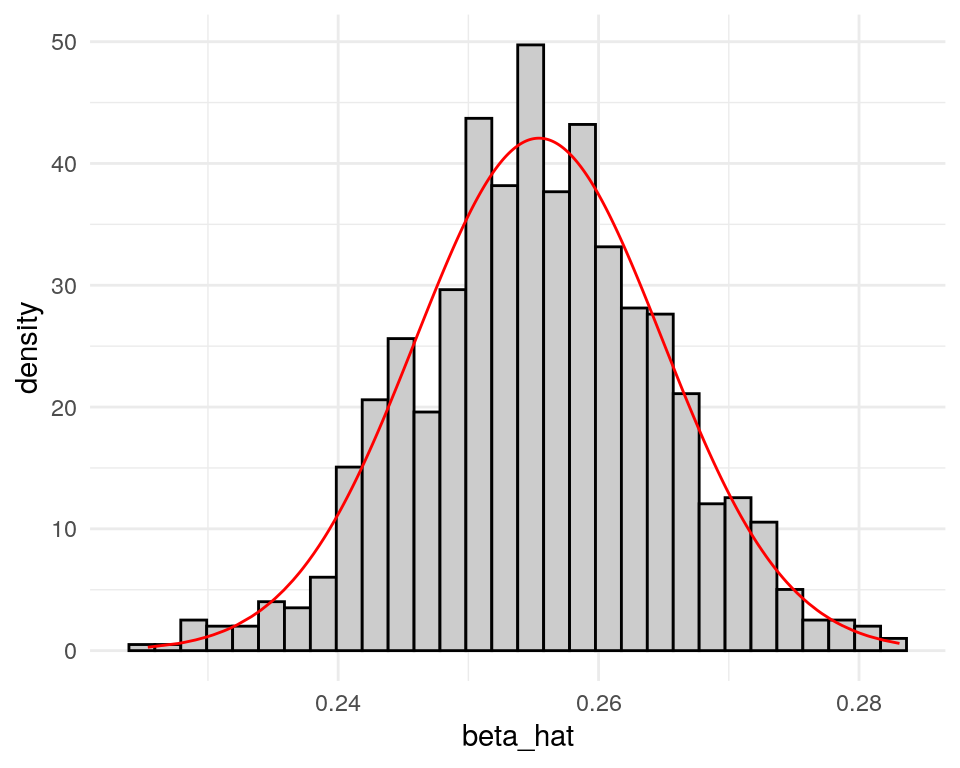
\includegraphics[width=0.55\linewidth]{RecEx9_files/figure-latex/unnamed-chunk-4-1}

\begin{Shaded}
\begin{Highlighting}[]
\NormalTok{dat =}\StringTok{ }\KeywordTok{data.frame}\NormalTok{(}\DataTypeTok{y =} \KeywordTok{factor}\NormalTok{(y), x)}
\end{Highlighting}
\end{Shaded}

To run cross-validation over a grid for \((C,\gamma)\), you can use a
two-dimensional list of values in the \texttt{ranges} argument:

\begin{Shaded}
\begin{Highlighting}[]
\NormalTok{r.cv <-}\StringTok{ }\KeywordTok{tune}\NormalTok{(svm, }\KeywordTok{factor}\NormalTok{(y) }\OperatorTok{~}\StringTok{ }\NormalTok{., }\DataTypeTok{data =}\NormalTok{ dat, }\DataTypeTok{kernel =} \StringTok{"..."}\NormalTok{, }\DataTypeTok{ranges =} \KeywordTok{list}\NormalTok{(}\DataTypeTok{cost =} \KeywordTok{c}\NormalTok{(...), }
    \DataTypeTok{gamma =} \KeywordTok{c}\NormalTok{(...)))}
\end{Highlighting}
\end{Shaded}

For the plot:

\begin{Shaded}
\begin{Highlighting}[]
\NormalTok{xgrid =}\StringTok{ }\KeywordTok{make.grid}\NormalTok{(x)}
\NormalTok{ygrid =}\StringTok{ }\KeywordTok{predict}\NormalTok{(..., xgrid)}
\KeywordTok{plot}\NormalTok{(xgrid, }\DataTypeTok{col =} \KeywordTok{as.numeric}\NormalTok{(ygrid), }\DataTypeTok{pch =} \DecValTok{20}\NormalTok{, }\DataTypeTok{cex =} \FloatTok{0.2}\NormalTok{)}
\KeywordTok{points}\NormalTok{(x, }\DataTypeTok{col =}\NormalTok{ y }\OperatorTok{+}\StringTok{ }\DecValTok{1}\NormalTok{, }\DataTypeTok{pch =} \DecValTok{19}\NormalTok{)}

\CommentTok{# decision boundary}
\NormalTok{func =}\StringTok{ }\KeywordTok{predict}\NormalTok{(..., xgrid, }\DataTypeTok{decision.values =} \OtherTok{TRUE}\NormalTok{)}
\NormalTok{func =}\StringTok{ }\KeywordTok{attributes}\NormalTok{(func)}\OperatorTok{$}\NormalTok{decision}
\KeywordTok{contour}\NormalTok{(}\KeywordTok{unique}\NormalTok{(xgrid[, }\DecValTok{1}\NormalTok{]), }\KeywordTok{unique}\NormalTok{(xgrid[, }\DecValTok{2}\NormalTok{]), }\KeywordTok{matrix}\NormalTok{(func, }\DecValTok{75}\NormalTok{, }\DecValTok{75}\NormalTok{), }\DataTypeTok{level =} \DecValTok{0}\NormalTok{, }
    \DataTypeTok{add =} \OtherTok{TRUE}\NormalTok{)  }\CommentTok{#svm boundary}
\end{Highlighting}
\end{Shaded}

\hypertarget{problem-5---optional-book-ex.-7}{%
\subsection{Problem 5 - optional (Book Ex.
7)}\label{problem-5---optional-book-ex.-7}}

This problem involves the OJ data set which is part of the ISLR package.

\begin{enumerate}
\def\labelenumi{(\alph{enumi})}
\item
  Create a training set containing a random sample of 800 observations,
  and a test set containing the remaining observations.
\item
  Fit a support vector classifier to the training data using
  \texttt{cost=0.01}, with Purchase as the response and the other
  variables as predictors. Use the \texttt{summary()} function to
  produce summary statistics, and describe the results obtained.
\item
  What are the training and test error rates?
\item
  Use the \texttt{tune()} function to select an optimal cost. Consider
  values in the range 0.01 to 10.
\item
  Compute the training and test error rates using this new value for
  cost.
\item
  Repeat parts (b) through (e) using a support vector machine with a
  radial kernel. Use the default value for \texttt{gamma}.
\item
  Repeat parts (b) through (e) using a support vector machine with a
  polynomial kernel. Set \texttt{degree=2}.
\item
  Overall, which approach seems to give the best results on this data?
\end{enumerate}

\hypertarget{refs}{}
\leavevmode\hypertarget{ref-ESL}{}%
Hastie, Trevor, Robert Tibshirani, and Jerome Friedman. 2009. \emph{The
Elements of Statistical Learning}. 2nd ed. Vol. 1. Springer series in
statistics New York.

\end{document}
